\documentclass[uplatex,12pt]{jsarticle}
\usepackage[dvipdfmx]{graphicx}
\usepackage{url}
\usepackage{listings,jlisting}
\usepackage{ascmac}
\usepackage{amsmath,amssymb}

%ここからソースコードの表示に関する設定
\lstset{
%  basicstyle={\ttfamily},
  basicstyle={\small},
  identifierstyle={\small},
%  commentstyle={\smallitshape},
%  commentstyle={\small\itshape},
  commentstyle={\small\ttfamily},
  keywordstyle={\small\bfseries},
  ndkeywordstyle={\small},
  stringstyle={\small\ttfamily},
  frame={tb},
  breaklines=true,
  columns=[l]{fullflexible},
  numbers=left,
  xrightmargin=0zw,
  xleftmargin=3zw,
  numberstyle={\scriptsize},
  stepnumber=1,
  numbersep=1zw,
  lineskip=-0.5ex
}
%ここまでソースコードの表示に関する設定

\title{知能プログラミング演習II 課題2}
\author{グループ8\\
  29114060 後藤 拓也\\
}
\date{2019年10月27日}

\begin{document}
\maketitle

\paragraph{提出物} rep2

\paragraph{グループ} グループ8

\paragraph{グループメンバー}
\begin{center}
\begin{tabular}{|c|c|c|}
  \hline
  学生番号&氏名&貢献度比率\\
  \hline\hline
  29114003&青山周平&no\\
  \hline
  29114060&後藤拓也&no\\
  \hline
  29114116&増田大輝&no\\
  \hline
  29114142&湯浅範子&no\\
  \hline
  29119016&小中祐希&no\\
  \hline
\end{tabular}
\end{center}
\paragraph{自分の役割} 必須課題2.1.(2)
\\ 「複数のパターンが与えられたときに全ての可能な変数束縛の集合を返すような\\プログラムの作成」
%%%%%%%%%%%%%%%%%%%%%%%%%%%%%%%%%%%%%%%%%%%%%%%%%%%%%%%%%%%%%%%%%%%%%%%%%%%%%%
\section{課題の説明}
\begin{screen}
複数のパターンが与えられたときに全ての可能な変数束縛の集合を返すようなプログラムを作成せよ.
例えば,上記の例で「?x is a boy」と「?x loves ?y」の両方が与えられたときに,(?x, ?y) の全ての可能な変数束縛の集合として{(Taro, Jiro), (Jiro, Hanako)}を返すこと.
\end{screen}

\section{手法}
課題を達成する(つまり, 「?x is a boy」と「?x loves ?y」と引数を取ると, {(Taro, Jiro), (Jiro, Hanako)}を返す)ために以下のようなプログラムの処理を行う.

\begin{enumerate}
\item 全体をまとめるハッシュマップを1つ生成する.
\item 1つ目の引数, 2つ目の引数を順番に処理を行う.
\item textファイルからデータセットを1行ずつ読み取り, 1行ずつ引数と照合する.
\item 1行はトークン単位に分割され, マッチングは各トークンごとで行う.
\item 対応した場合, ハッシュマップにKeyとして変数(?xや?yなど)を, Valueとして具体定数(TaroやJiroなど)を加えていく.
\item 1つ目の引数で束縛された変数は, 2つ目の引数に反映される(1つ目で?x=Taroと決まれば, 2つ目の引数ではその条件を引き継がせる).
\item ハッシュマップを2次元リストにし, 中身(Keyや各Keyに対応するVlaue)をリスト化することで, 全てのマッチング可能なパターンを1つのハッシュマップに格納できる.
\end{enumerate}

\begin{figure}[htbp]
 \begin{center}
  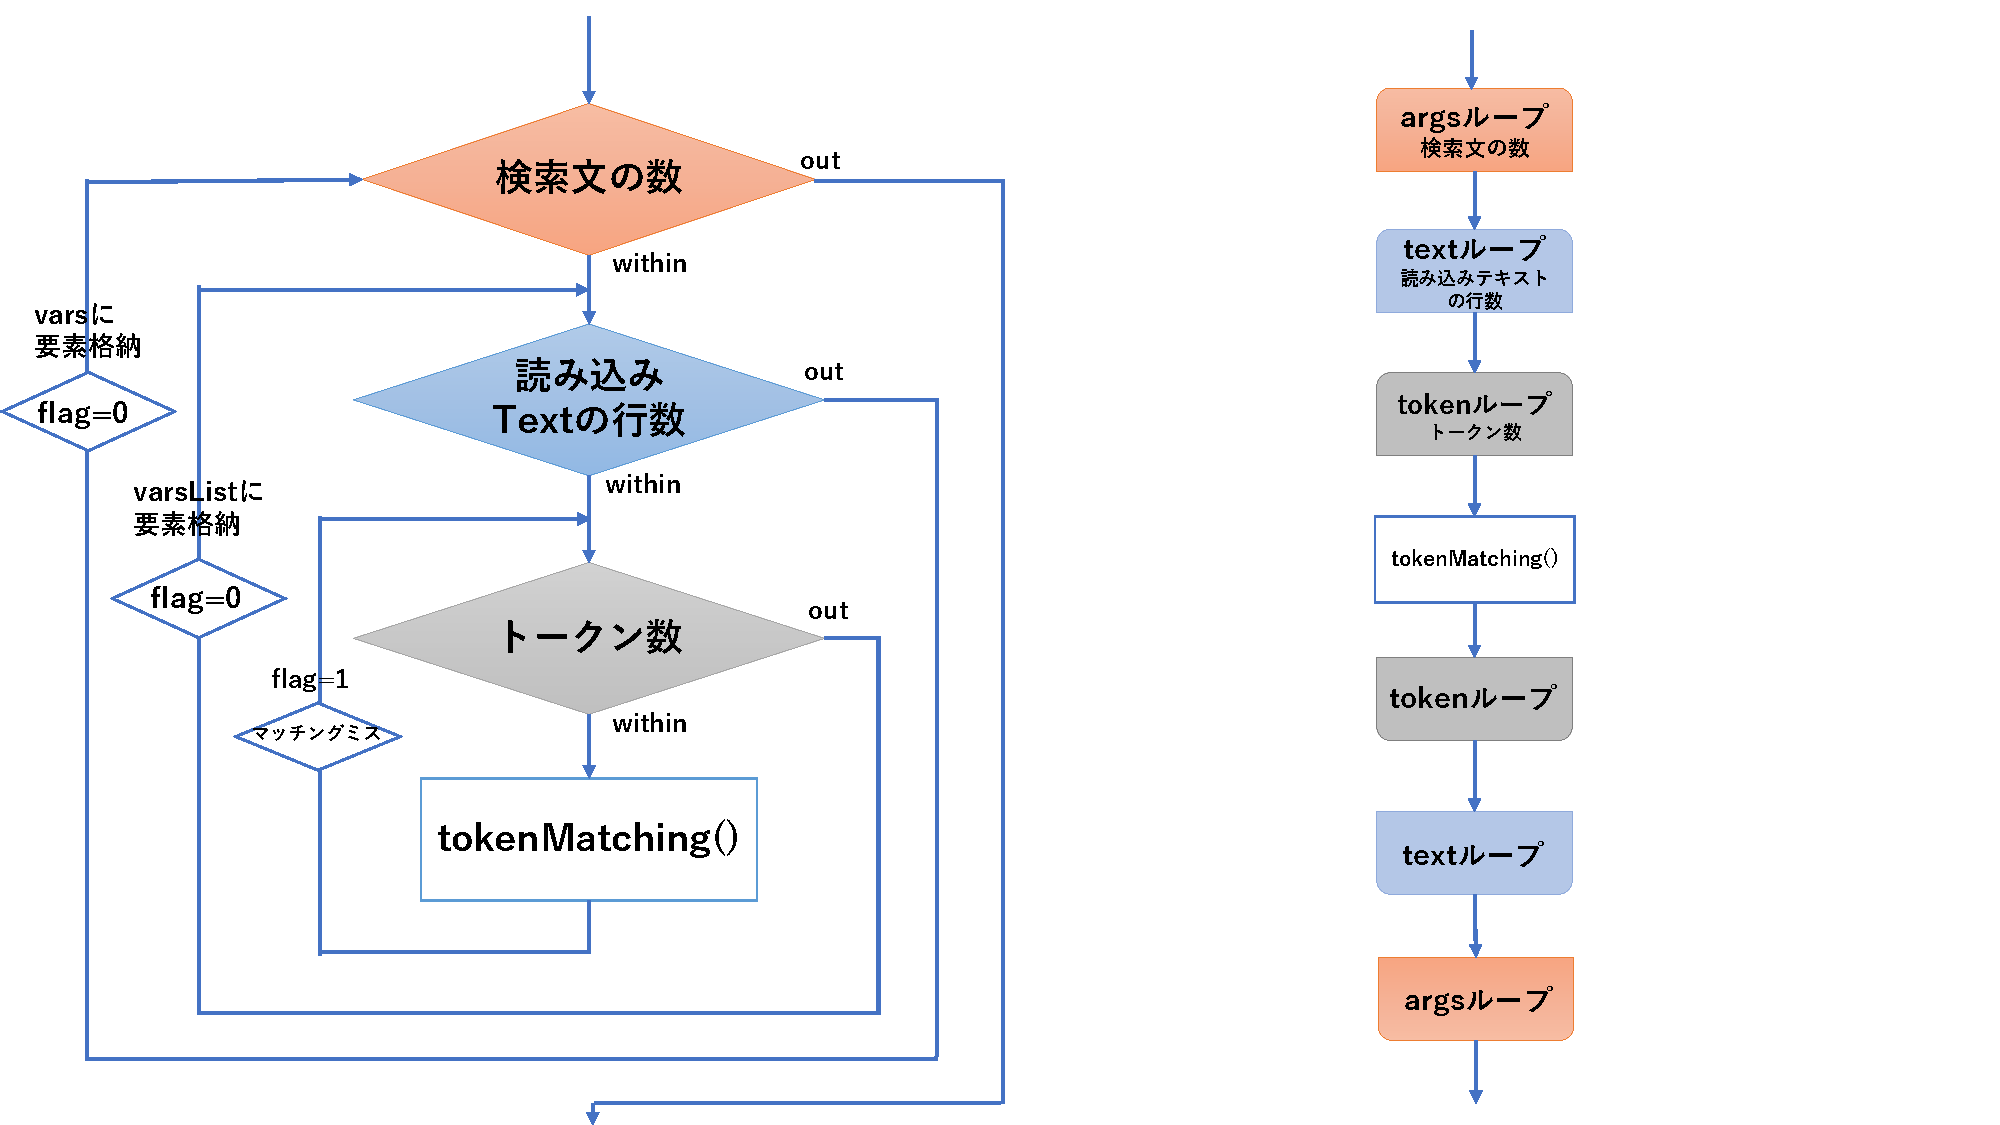
\includegraphics[width = 10cm, pagebox = cropbox, clip]{unify構造.pdf}
 \end{center}
 \caption[]{unifyプログラムの3つのループ}\label{fig:fig1.1}
\end{figure}

プログラムの流れは多段階のループ構造を構築している. 図1における"3つの大きなループ"を参照し, 上記の7つの手法について詳しく説明する.

1.に関して, mainクラスで1度Unifierクラスのインスタンスが生成されるとコンストラクタにより, ハッシュマップをはじめとするあらかじめ宣言されていた複数の変数やリストを初期化する. ここで初期化され生成されたインスタンスは, 今後のプログラム全体で使われる.

2.に関しては, 2つの引数をリストに格納させ, ループ処理を行う. ここが1つ目の大きなループである.

3.に関しては, BufferedReaderオブジェクトによりテキストを1行ずつ読み込む. ここが2つ目の大きなループである.

4.に関しては, 既存のプログラムを利用し, StringTokenizerにより分解したトークンの数だけループ処理をする. ここが3つ目の大きなループである. 引数と読みこんだ1行とでトークン数の異なる場合は, トークン数の多いほうにそろえるように, 少ないほうにnullを入れて数を調整する.

5.に関しては, トークン単位のマッチングは成功しても, 1行を通して成功していなければ成功とはいえない. 例えば, 「?x is a boy」と「Hanako is girl」は, トークン単位のループ処理ででマッチングをしていくと, 先に「?x = Hanako」でマッチングが成功するが, その後「boy != girl」となるので, 今回は失敗であり, ハッシュマップには追加できない. これを実現するために, 1行すべてのマッチングが成功した後に, これまで成功していたトークンの組をハッシュマップに保存する処理を行う. 具体的には, マッチングが成功したトークンの組はそれぞれ一時バッファならぬ一時リストに追加して, ハッシュマップには追加しない. マッチングの成功不成功を判断する"ミスフラグ"を用意し, 1行におけるトークンの組み合わせすべてが成功したら(ミスフラグが上がらなかったら), 先ほどの一時リストの要素をハッシュマップに保存する.

6.に関しては, 「?x = Taro, Jiro」と1つの変数において, 2つの定数が束縛されることがあるので, それぞれにおいて2つ目の引数を変更する. 具体的には, 2つ目の引数は「?x loves ?y」から「Taro loves ?y」と「Jiro loves ?y」の2つに変更させる. そのため, 手法1説明したで1つ目の大きなループは, 引数2つであっても, 3回ループが行われる.

7.に関しては, 上記の手法6で述べたように, 1つのKey(たとえば?x)に対して, 複数のValue値{Taro, Jiro}を持つので, リスト化する必要があった. 上記の手法6で"トークン(語)の単位で行うのではなく, 1行単位でハッシュマップに保存をする"と述べたが, この際, 実際のマップに保存するわけではなく, 2次元リストであるハッシュマップに格納するためのリストに保存している.

\section{実装}
上記の7つの手法の中で, 特に重点を置いた箇所に関して, プログラムを参照にしつつ説明していく.

手法5に関する「1行を通してすべてのトークンがマッチングに成功した時のみ, ハッシュマップに反映させる」の部分を実装したソースコード\ref{src:No1}に示す。
\begin{lstlisting}[caption=1文すべて終わったら格納する,label=src:No1]

  for(int i = 0 ; i < length ; i++){ //1語ずつマッチングしていきます
	System.out.println("flag = " + flag);

	if(!tokenMatching(buffer1[i],buffer2[i])){ //マッチングできてないなら...
		System.out.println("Search Error 2");

		flag = 1;  //missフラグ上げる
	}

  } //1文の解析がすべて終わって...
  if(flag == 0) {	//missflagが一度も上がっていないなら,
	for(int len = 0; len < ValueList.size(); len++) {
	    //HashMapに格納せずに,
	    //vars.put(KeyList.get(len), ValueList.get(len));
	    System.out.println("ValueList.get("+ len + ") ="+ValueList.get(len));

	    //varslistに格納
	    varslist.add(ValueList.get(len));
	}
  } //Textの文全てが終わったら...
\end{lstlisting}

flagはフィールド変数として, Unifierクラスのどのメソッドでも用いられる. 上記には書かれていないが, tokenMatchingメソッドのvarMatchingメソッド内で1単語(トークン)をマッチングさせるたびに, マッチング成功の成否に合わせflag管理をしている.

また, ハッシュマップは実際には2次元リストにより構築されているため, 1文解析がすべて終わり, フラグが立ってない場合の処理だが, 手法5の説明時には簡略化のために省略したが, 実際には"ハッシュマップに格納する"のではなく, "ハッシュマップに格納するためのリストvarslistに登録する"である.\\\\

手法6に関する「1つ目の引数により得られた束縛条件を2つ目の引数に反映する」の部分を実装したソースコード\ref{src:No2}に示す。

\begin{lstlisting}[caption=第1引数から第2引数への変数束縛条件の引継ぎ ,label=src:No2]
//1つ目の引数,2つ目の引数,順番に処理する!
for(int num = 0; num < args.size(); num++) {

   if(num == 1) {  //2回目で
      //変数(?x,?yなどなど)の数だけ...
      for(int keyNum = 0; keyNum < KeyList.size(); keyNum++) {
          //その変数に対応する値(Taro, Jiroなどなど)の数だけ
          for(int valueNum = 0; valueNum < varslist.size(); valueNum++) {

    		//文字列の中に?が入っていたら...
    		if(string2.contains("?")) {
    			//文字列として置き換えて,新しく作成!
    			String stringx = string2.replace(KeyList.get(0), varslist.get(valueNum));
    			System.out.println("stringx = " + stringx);
    			args.add(stringx);	//などなど
    		}
    	   }
    	}
    	args.remove(1); //もとを置き換え
    	System.out.println("args.size() = " + args.size());
    }	
     
    varslist = new ArrayList<String>();   //複数人対応のValue:値を格納させる.
\end{lstlisting}

1つ目のマッチングの結果で得られたKeyを格納したKeyList, 各Keyに対応したValueを格納したvarslistが用いられている. 具体的には, 1つ目の引数で"?x is a boy"としたとき, ?x = Taro, Jiroが当てはまるため, KeyListには「?x」が, varslistには「Taro, Jiro」が含まれている. これをreplaceメソッドを用いて, 実際に「?xをTaro」という風におきかえている.

ポイントとしては, 引数は2つでも, 1つ目の引数のマッチングの結果, 「?x = Taro, Jiro」のように複数対応する場合, 2つ目の引数が「?x loves ?y」の際, ?xが2つ代入され, 「Taro loves ?y」と「Jiro loves ?y」と増えることである. そのため, 元あった「?x loves ?y」を消すために. removeメソッドで代入前の1文を消している.\\\\\\


手法7に関する「ハッシュマップの2次元リスト化による要素代入」の部分を実装したソースコード\ref{src:No3}に示す。
\begin{lstlisting}[caption=ハッシュマップの2次元リスト化,label=src:No3]
   if(flag == 0) {

      //いま見てるKeyの番号にしないと!
	int index = KeyList.indexOf(String.valueOf(keyList.get(0)));
	System.out.println("KeyList = " + KeyList.get(index));
	
	/* 参照渡しだから,作ったリストを削除してももとの場所をささない.*/
	ArrayList<String> array = new ArrayList<>();
	if(vars.containsKey(KeyList.get(index))) {	//すでに作ったことがあったら,
	    System.out.println("削除します");
	    array.clear();	//消す
	    array = arrayCopy;//コピーを戻す
		   flag2 = 1;
	}
	arrayCopy = array;	//コピーを取っておいて,
	array.add(ValueList.get(0));
	if(flag2 == 0)
	     vars2list.add(array);
	System.out.println("vars2list() = " + vars2list.toString());
	vars.put(KeyList.get(index), vars2list.get(index));  //改良HashMapに格納

	flag2 = 0;
   }
    System.out.println("途中結果は" + vars.toString() + "\n");
    flag = 0; //falgのリセット
\end{lstlisting}

ここの処理はTextの全ての行が読み込めたら行われる. 2次元リストを作るためには, リストに格納する処理を行うが, その際, Keyの数(?xだけなら1つ, ?xと?yなら2つなど)に応じて, 複製するValueのリストの数も変わってくる. リストの名前には, 配列のbuffer[i]のように数字を名前に付け加えることができないため, ループ処理を行うこのプログラム中では, とりあえず, リストを作成するが, すでにあるKeyに対してリストが存在していれば, ダブってしまうので, 削除する. このとき, javaではリストのオブジェクトも参照渡しであるので, ただ消すだけでは, 参照先を前のリストに戻すことができない. そのために, 前のリストをコピーしておき, 消した際には, コピーもとを参照させる.\\\\\\

\begin{lstlisting}[caption=複数候補に対応したvarMatchingメソッド,label=src:No4]
boolean varMatching(String vartoken,String token){
  /* (注意)
    * すでに?x=Taroという制約がある状態で,さらに?x=Jiroを付け加えないといけない. うやむやにやっても,かぶっている候補を増やしてしまうだけである. */
 //すでにあるKeyに対して...
    //HashMapにvartokenというキー(Not値)が存在するかどうか
    if(vars.containsKey(vartoken)){
    	  System.out.println("varslist.size() = " + varslist.size());

    	  //まだvarslistには入ってないけど,Maticng成功した場合,
    	  if(varslist.size() == 0) {
      		  ValueList.add(token);
      		  keyList.add(vartoken);
    	  }
    	  //普段はこっちだよね
    	  else {
    	  	for(int i = 0; i < varslist.size(); i++) {
    		    //すでに登録されている関係なら...
    		    if(token.equals((vars.get(vartoken)).get(i)))
    			  System.out.println("格納済み");
          	    else { //別の値(TaroじゃなくてJiro)が来たら, 加えます.
          		  ValueList.add(token);
          		  keyList.add(vartoken);  //Keyも含めて再登録しないと...
         	    }
    	  	}
    	  }
    	  return true;
    }

  //初めてのKeyに関して...
    else {
          replaceBuffer(vartoken,token);
          //HashMapの値リスト:varslistに含まれているかどうかで見る
          if(varslist.contains(vartoken)) {
              replaceBindings(vartoken,token);
          }
          //vars.put(vartoken,token);  //ここではハッシュマップに登録しません.
          if(!KeyList.contains(vartoken)) {   //1回だけでっせ!
        	  KeyList.add(vartoken);
          }
          ValueList.add(token);
          keyList.add(vartoken);
    }
    return true;
}
\end{lstlisting}

上記は, 実際に1(トークン)単語単位でマッチングを行うvarMatchingメソッドである. ValueListとkeyListは, テキストの1行ずつで初期化されるようになっており, ここのメソッド内でしかこの2つのリストは操作されない. この1行単位で初期化されるリストの結果は, 全体に反映されるリストvarslistに別のメソッドで格納されるので, それをもとにif文の条件分岐を行っている.

\section{実行例}
引数に["?x is a boy, ?x loves ?y"]としたときの実行結果が以下のようになる.
\begin{lstlisting}
Successfully started
検索結果を取得
★answer = ?x0 = Taro
★answer = ?y0 = Jiro
★answer = ?x1 = Jiro
★answer = ?y1 = Hanako
\end{lstlisting}

?xには, Taro, Jiroが入り, その後, 2つ目の引数は「Taro loves ?y」, 「Jiro loves ?y」と置き換えられ, ?yはJiro, Hanakoが入る. 出力結果を, それぞれのxとyに対応させるために, ハッシュマップから, KeyとValueのfor文を回している.

正しい関係性が出力されていることが確認される.

同様に, ["?x is a student, ?x studies ?y"]と実行すると,
\begin{lstlisting}
Successfully started
検索結果を取得
★answer = ?x0 = Hanako
★answer = ?y0 = philosophy
★answer = ?x1 = Taro
★answer = ?y1 = informatics
\end{lstlisting}
と出力されることが確認された.


\section{考察}
6に関して, 1つ目の引数で束縛された変数の値を, 実際に2つ目の引数に代入するので, もし「?x loves ?y」と「?x is a boy」という順番の引数の組み合わせだと最終的に間違ったハッシュマップが生じる. というのも, 「?x loves ?y」にあたる?xは[Hanako, Taro, Jiro]であるので, ハッシュマップその組み合わせが登録されるが, 「Hanako is a girl」なので, ミスが生じるが既にハッシュマップに登録されているので間違った出力となる.
これはunifyしていない. ただのMatchingである....
引数も2つに限定させてしまった.


\section{感想}
まじで難しかった.
変数の大文字小文字がかなりザツでプログラム作成の後半になればなるほどわかりにくかった.

%%%%%%%%%%%%%%%%%%%%%%%%%%%%%%%%%%%%%%%%%%%%%%%%%%%%%%%%%%%%%%%%%%%%%%%%%%%%%%
% 参考文献
\begin{thebibliography}{99}
\bibitem{notty} Javaによる知能プログラミング入門 --著:新谷 虎松 \\
\bibitem{notty} java CSV出力 --著:TECH Pin \\
\url{https://tech.pjin.jp/blog/2017/10/17/【java】csv出力のサンプルコード}
\end{thebibliography}

\end{document}